\chapter{Basics on Statistical Mechanics of simple systems}

\section{Curie-Weiss Model}
\noindent
El modelo de Curie-Weiss describe un sistema de $N$ "spins" (que en nuestro ámbito representarán neuronas) que pueden estar en dos estados: $\sigma_i \in \{+1, -1\}$, equivalentes a una neurona activa o en reposo. \\

\noindent
La característica clave del modelo de Curie-Weiss es que es un modelo de campo medio (Mean Field). Esto significa que cada neurona interactúa con todas las demás de la red con la misma intensidad, sin importar la distancia o la geometría. Es lo que llamamos un ``grafo completo''. \\


\begin{definicion}[Hamiltoniano del Modelo de Curie-Weiss]
    El \tbf{Hamiltoniano} (Función de Energía) define la energía total del sistema para una configuración dada de estados $(\sigma)$. En el modelo CW, se define como:
    $$ \mathcal{H}_{N,J,h}(\sigma) = - \sum_{i, j} \sigma_i J_{ij}\sigma_j - \sum_{i=1}^{N} h_i\sigma_i $$
    donde $J_{ij} = \dfrac{J}{N}$ para todo par $(i,j)$, es decir, todas las neuronas están igualmente conectadas con un peso $J/N$, y $h_i=h \ \forall i$, por lo que otra definición equivalente es:
    \begin{equation*}
        \mathcal{H}_{N,J,h}(\sigma) = - \frac{J}{N} \sum_{i > j} \sigma_i \sigma_j - h \sum_{i=1}^{N} \sigma_i
    \end{equation*}
    notar que el primer sumatorio debería ser el doble, pues solo cuenta cada par una vez  y no las autointeracciones (de ahí la condición $i>j$), pero aún así es una definición válida. Las características son las siguientes:
    \begin{itemize}
        \item $J$: Es la constante de acoplamiento. Si $J > 0$, el sistema es ferromagnético: las neuronas prefieren estar alineadas (todas activas o todas inactivas) porque eso minimiza la energía.
        \item $h$: Representa un campo externo (un estímulo sensorial o sesgo) que empuja a las neuronas hacia un estado específico.
        \item $1/N$: Es un factor de escala necesario para que la energía sea "extensiva" (que crezca linealmente con el número de neuronas).
    \end{itemize}
\end{definicion}

\noindent
Para simplificar el análisis de $N$ variables, introducimos una variable macroscópica llamada \tbf{magnetización} ($m$), que mide el promedio de actividad de la red
\begin{equation*}
    m_N(\sigma) = \frac{1}{N} \sum_{i=1}^{N} \sigma_i
\end{equation*}
que toma valores en $M_N = \{1 - 2i/N, i = 1, ..., N \}$, donde si $m_N(\sigma) = 1 - 2i/N$ entonces la configuración $\sigma$ tiene $i$ espines hacia abajo y $N - i$ hacia arriba. Ahora podemos reescribir el Hamiltoniano en términos de la magnetización
\begin{equation*}
    \mathcal{H}_{N,J,h}(\sigma) = - \frac{NJ}{2} [m_N(\sigma)]^2 +-hN m_N(\sigma) +\dfrac{J}{2}=N\phi_{J,h}(m_N(\sigma))
\end{equation*}
donde lo que hemos hecho es lo siguiente:
\begin{align*}
    &\left( \sum_{i=1}^N \sigma_i \right)^2 = \sum_{i=1}^N \sum_{j=1}^N \sigma_i \sigma_j \overset{(*)}{\implies} (Nm_N(\sigma))^2 = \sum_{i=1}^N \sigma_i^2 + 2 \sum_{i>j} \sigma_i \sigma_j \implies \\
    &\implies \sum_{i>j} \sigma_i \sigma_j = \frac{(Nm_N(\sigma))^2 - N}{2} = \frac{N^2 [m_N(\sigma)]^2 - N}{2}
\end{align*}
donde en $(*)$ hemos usado que cuando $i=j$, $\sigma_i^2 = 1$, por lo que $\sum_{i=1}^N \sigma_i^2 = N$, y para pares $i\neq j$ contamos cada par dos veces por ser simétrica ($\sigma_i \sigma_j$ y $\sigma_j \sigma_i$), por lo que hay exactamente el doble de términos que en el sumatorio $i > j$, es decir $2 \sum_{i>j} \sigma_i \sigma_j$. \\
\noindent       
Finalmente sustituimos en el Hamiltoniano el término $\sum_{i>j} \sigma_i \sigma_j $, de la siguiente forma:
\begin{align*}
    \mathcal{H}_{N,J,h}(\sigma) &= - \frac{J}{N} \sum_{i > j} \sigma_i \sigma_j - h \sum_{i=1}^{N} \sigma_i = - \frac{J}{N} \cdot \frac{N^2 [m_N(\sigma)]^2 - N}{2} - hN m_N(\sigma) = \\
    &= - \frac{NJ}{2} [m_N(\sigma)]^2 - hN m_N(\sigma) +\dfrac{J}{2}
\end{align*}
Como es lógico $J$ puede ser tanto positiva como negativa, pero en el contexto de redes neuronales y sistemas biológicos, generalmente se asume que $J > 0$ (\tbf{ferromagneto}), ya que las neuronas tienden a activar a otras neuronas similares (excitación mutua) en lugar de inhibirse entre sí, es decir, si la neurona $i$ está encendida ($+1$), empuja a su vecina $j$ a encenderse también para que el producto $\sigma_i \sigma_j$ sea positivo. Esto minimiza el término $-J \sigma_i \sigma_j$ en el Hamiltoniano. En redes neuronales, esto es lo que permite crear atractores (recuerdos estables). \\

\noindent
El caso $J < 0$ correspondería a un sistema antiferromagneto, donde las neuronas tienden a estar en estados opuestos (una activa y la otra inactiva). Este tipo de interacción es menos común en modelos de redes neuronales, pero podría representar situaciones donde la inhibición mutua es dominante. \\

\noindent
El modelo de Curie-Weiss, usa como ya hemos comentado $J>0$. Este modelo no nos indicará cómo evolucionan las neuronas en el tiempo, sino que nos dará información sobre las configuraciones de equilibrio del sistema, es decir, cuáles son las configuraciones más probables de encontrar en función de los parámetros $J$, $h$ y la temperatura $T$, mediante la siguiente distribución de probabilidad
\begin{equation*}
    \rho_{N,J,h,\beta}(\sigma) = \frac{e^{-\beta \mathcal{H}_{N,J,h}(\sigma)}}{Z_{N,J,h,\beta}} \quad \text{ tal que } \quad Z_{N,J,h,\beta} = \sum_{\sigma} e^{-\beta \mathcal{H}_{N,J,h}(\sigma)}
\end{equation*}
donde tenemos que 
\begin{itemize}
    \item La expresión $e^{-\beta H}$ representa la \tbf{exponencial de Boltzmann} que es la lógica central. Los estados con menor energía ($H$ muy negativo) tienen una probabilidad mucho más alta de ocurrir. La red ``cae'' en los valles de energía (que son nuestros patrones memorizados).
    \item La función $Z$ es la \tbf{función de Partición}, que matemáticamente es solo una constante de normalización (la suma de todos los pesos exponenciales posibles) para que la probabilidad total sume 1.
\end{itemize}

\subsection{Thermodynamic observables}
A continuación veremos algunas funciones importantes que nos ayudarán a entender el comportamiento del sistema
\begin{itemize}
    \item La \tbf{Energía Libre} ($F$) y la \tbf{Energía Libre Intensiva} ($f$), dadas por
    \begin{equation*}
        F_{N,J,h,\beta} = -\frac{1}{\beta} \log Z_{N,J,h,\beta} \quad \text{y} \quad f_{N,J,h,\beta} = \frac{F_{N,J,h,\beta}}{N}
    \end{equation*}
    donde la energía libre $F$ mide el equilibrio entre energía y entropía (desorden) del sistema, y la versión intensiva $f$ nos da esta medida ``por neurona'', útil para comparar sistemas de diferentes tamaños. \\

    \noindent
    Cuando hablamos de que la energía libre y libre intesiva, representan el equilibrio entre energía y entropía, nos referimos a que el sistema siempre busca minimizar su energía (bajar $H$) buscando estados ordenados (como todos los espines hacia arriba o hacia abajo), pero al mismo tiempo, la entropía (que mide el desorden) tiende a maximizarse, ya que aunque estos estados desordenados tienen baja energía, son muchos en la cantidad, por lo que al sumar sobre todas las configuraciones, la estadística empieza a ganar por "cantidad" lo que pierde por "calidad" (energía).

    \item La \tbf{Energía Libre en el Límite Termodinámico} ($f_{\beta, J, h}$)
    \begin{equation*}
        f_{\beta,J,h} = \lim_{N \to \infty} f_{N,J,h,\beta}    
    \end{equation*}
    que es el valor de la energía libre cuando tenemos una red ``infinita''. En matemáticas de redes neuronales, solo cuando $N \to \infty$ aparecen los fenómenos de fases (como el paso de ``no recordar nada'' a ``recordar perfectamente''). Estudiamos este límite porque las redes reales tienen miles de millones de conexiones y se comportan de forma muy similar al límite infinito.
    \item La \tbf{Presión Intensiva} ($A_{N,J,h,\beta}$), dada por 
    \begin{equation*}
        A_{N,J,h,\beta} = \frac{1}{N} \log Z_{N,J,h,\beta}
    \end{equation*}
    es simplemente otra forma de escribir la energía libre (fíjate que $A_{N,J,h,\beta} = -\beta f_{N,J,h,\beta}$). Se suele usrr mucho porque es más manejable para usar técnicas como el ``interpolatión trick'' o el ``replica trick''. Representa lo mismo: el estado de equilibrio del sistema. \\
    \noindent
    Al igual que antes, definimos la \tbf{Presión Intensiva en el Límite Termodinámico} ($A_{\beta,J,h}$)
    \begin{equation*}
        A_{\beta,J,h} = \lim_{N \to \infty} A_{N,J,h,\beta}
    \end{equation*}
    \item El \tbf{Promedio Térmico de un Observable} ($\omega_{N,J,h,\beta}$), dada por
    \begin{equation*}
        \omega_{N,J,h,\beta}(g) = \sum_{\sigma} g(\sigma) \rho_{N,J,h,\beta}(\sigma)
    \end{equation*}
    es una función que nos permite calcular el valor esperado de cualquier cosa que queramos medir ($g$) en la red bajo la distribución de probabilidad $\rho_{N,J,h,\beta}$. Viene a ser esperanza ponderada por $g$ y la probabilidad $P$. \\
    \noindent
    Si quieres saber, por ejemplo, cuál es la magnetización promedio ($m$) de la red, no miras una foto fija, sino que haces un promedio pesado por la probabilidad $P$ de todos los estados. En nuestros apuntes, veremos que a menudo se escribe como $\langle g \rangle$. Es lo que se vería si observaramos la red durante mucho tiempo bajo un nivel de ruido constante (temperatura fija).
\end{itemize}

\noindent
Ahora estudiaremos la función de partición $Z_{N,J,h,\beta}$ para reducir la sumatoria, pues si tenemos una red neuronal con muchas neuronas, es decir, $N$ grande, la sumatoria se vuelve inabarcable, ya que existen $2^N$ configuraciones posibles. Para ello, usaremos la variable macroscópica magnetización $m_N(\sigma)$ que ya hemos definido antes. Notar que muchas configuraciones diferentes $\sigma$ pueden tener la misma magnetización $m$, por lo que podemos reagrupar la sumatoria en $Z$ según los valores de $m$, veámoslo

\begin{equation*}
    Z_{N,J,h,\beta} = \sum_{\sigma} e^{-\beta \mathcal{H}_{N,J,h}(\sigma)} = \sum_{m \in M_N}  e^{-\beta \mathcal{H}_{N,J,h}(\sigma)} \Omega_N(m)
\end{equation*}
donde $\Omega_N(m)$ es el número de configuraciones $\sigma$ que tienen una magnetización $m$, es decir, la \tbf{densidad de estados} con magnetización $m$. Esta cantidad se puede calcular combinatoriamente, ya que si $m = 1 - 2i/N$, entonces hay $i$ espines hacia abajo y $N-i$ hacia arriba, por lo que
\begin{equation*}
    \Omega_N(m) = \binom{N}{i} = \binom{N}{\frac{N(1-m)}{2}}
\end{equation*}
usando la definición del coeficiente binomial (más adelante veremos la demostración de la segunda igualdad). A continuación, definiremos la entropía $S_N(m)$ como el logaritmo natural de la densidad de estados
\begin{equation*}
    S_N(m) = \log \Omega_N(m)
\end{equation*}
teniendo por tanto 
\begin{equation*}
    Z_{N,J,h,\beta} = \sum_{m \in M_N}  e^{-\beta \mathcal{H}_{N,J,h}(\sigma)} e^{S_N(m)}= \sum_{m \in M_N}  e^{\beta \left[ -\mathcal{H}_{N,J,h}(\sigma) + TS_N(m) \right]}= \sum_{m \in M_N}  e^{-\beta F_N(m)}
\end{equation*}
donde hemos definido la \tbf{Energía Libre de Helmholtz} ($F_N(m)$) como
\begin{equation*}
    F_N(m) = \mathcal{H}_{N,J,h}(\sigma) - TS_N(m)
\end{equation*}
que mide el equilibrio entre energía y entropía para una magnetización $m$ dada. La red neuronal vive en una competencia constante. La energía quiere orden y memoria, mientras que la entropía (potenciada por la temperatura $T$, es decir, $T\cdot S$) quiere caos y ruido. El sistema siempre buscará el estado $m$ que minimice esta competencia ($F$). \\

\subsection{Saddle Point Method(or Laplace's Method)}
\noindent
Lo que intentaremos buscar en esta resolución es encontrar a partir de que valor $T$ (ruido) la red deja de recordar el patrón almacenado. Para ello, usaremos el \tbf{Método del Punto de Silla} (o \tbf{Método de Laplace}), que nos permite aproximar sumas o integrales de funciones exponenciales cuando $N$ es grande. La idea clave es que, para $N$ grande, la suma está dominada por el término donde el exponente es máximo (o mínimo si es negativo). \\

\noindent
En primer lugar, tenemos que la probabilidad de observar una magentización especifica $\tilde{m}$ en la red es
\begin{equation*}
    \rho_N(\tilde{m}) = \sum_{\sigma} \rho_N(\sigma) \delta(\tilde{m} - m_N(\sigma))
\end{equation*}
donde $\delta$ es la delta de Kronecker, que selecciona solo las configuraciones $\sigma$ que tienen magnetización $m_N(\sigma) = \tilde{m}$. Al final, $\rho_N(\tilde{m})$ es simplemente la suma de las probabilidades de todas aquellas configuraciones que "votan" por el mismo valor de memoria. \\

\noindent
En lo siguiente, utilizaremos la notación $m$ para referirnos a una magnetización genérica $\tilde{m}$, y $m_N(\sigma)$ para la magnetización específica de una configuración $\sigma$. \\

\noindent
Ahora, veremos una igualdad importante que nos permitirá simplificar la expresión de $p_N(m)$, usando una función cualquiera $g$, veámoslo
\begin{align*}
    &\sum_{m\in M_N} \rho_N(m) g(m) = \sum_{m\in M_N}g(m) \sum_{\sigma} \rho_N(\sigma) \delta(m - m_N(\sigma)) = \sum_{\sigma} \rho_N(\sigma) \sum_{m\in M_N}g(m) \delta(m - m_N(\sigma))= \\
    &\overset{(*)}{=} \sum_{\sigma} \rho_N(\sigma) g(m_N(\sigma))=\omega_N(g(m_N(\sigma)))
\end{align*}
donde en $(*)$ hemos usado la propiedad de la delta de Kronecker, que selecciona el valor $m = m_N(\sigma)$ en el sumatorio, de manera que $g(m)$ solo contribuye cuando $m = m_N(\sigma)$. \\

\noindent
Calculemos finalmente $\rho_N(m)$ usando la igualdad anterior con $g(m) = \delta(m - \hat{m})$, veámoslo
\begin{align*}
    \rho_N(m) = \sum_{\sigma} \rho_N(\sigma) \delta(m - m_N(\sigma))\overset{(*)}{=}\sum_{\sigma} \left[ \frac{1}{Z_N} e^{-\beta H_N(\sigma)} \right] \delta(m - m_N(\sigma))=\dfrac{Z_n(m)}{Z_N}
\end{align*}
donde en $(*)$ hemos usado la forma de Boltzmann de la distribución de probabilidad $\rho_N(\sigma)$, es decir
\begin{equation*}
    \rho_N(\sigma) = \dfrac{e^{-\beta H_N(\sigma)}}{Z_N}
\end{equation*}
Tenemos por tanto que
\begin{equation*}
    Z_N(m) = \sum_{\sigma} \delta(m - m_N(\sigma)) e^{-\beta H_N(\sigma)}
\end{equation*}
es la \tbf{función de partición restringida} a una magnetización $m$. Además
\begin{equation*}
    \rho_N(m) = \dfrac{Z_N(m)}{Z_N} = e^{-\beta (F_N(m) - F_N)}
\end{equation*}
donde 
\begin{equation*}
    F_N(m) = -\frac{1}{\beta} \log Z_N(m)
\end{equation*}
es la \tbf{energía libre restringida} a una magnetización $m$. Análogamente, definimos la \tbf{energía libre intensiva restringida} como
\begin{equation*}
    f_N(m) = \frac{F_N(m)}{N}
\end{equation*}

\noindent
Antes de avanzar es importante tener claro el significado físico de estas cantidades:
\begin{itemize}
    \item $Z_N(m)$: Nos dice cuánto "peso" tienen todas las configuraciones con magnetización $m$. Es como si filtráramos todas las posibles configuraciones y solo miráramos aquellas que tienen un nivel específico de memoria (magnetización).
    \item $F_N(m)$: Mide el equilibrio entre energía y entropía para las configuraciones con magnetización $m$. Nos dice qué tan "favorable" es ese nivel de memoria en términos de energía libre.
    \item $\rho_N(m)$: Es la probabilidad de encontrar la red en un estado con magnetización $m$. Nos indica qué tan probable es que la red recuerde un patrón con un cierto nivel de fidelidad.
\end{itemize}

\begin{observacion}
    Cuando hablamos en este concepto de una función ``restringida'' nos referimos a que hemos limitado la consideración a un subconjunto específico de todas las configuraciones posibles del sistema, en este caso, aquellas que tienen una magnetización fija $m$. Esto nos permite analizar el comportamiento del sistema bajo condiciones específicas, en lugar de considerar todas las configuraciones posibles de manera indiscriminada.
\end{observacion}

\noindent
A partir de ahora, no necesitaremos calcular $Z_N$ directamente, es decir, todas las configuraciones posibles, sino que nos centraremos en $Z_N(m)$, que es mucho más manejable. La idea de esto, es que podemos representar cuánta importancia tiene un valor concreto de memoria para el sistema, por lo que si $Z_N(0.8)$ es mucho más grande que $Z_N(0)$, la red nos está diciendo que ``prefiere'' con mucha diferencia estar en un estado de alta memoria que en uno de ruido (recordemos que el caso $m=0$ es ruido total, sin memoria). \\

\noindent
Estudiemos ahora el caso más sencillo donde $f_N(m)$ tiene un único mínimo global en $m=m^*$. en este caso, tomando el desarrollo de taylor de $f_N(m)$ alrededor de $m^*$, tenemos
\begin{equation*}
    f_N(m) \approx f_N(m^*) + f_N'(m^*)(m - m^*) + \frac{1}{2} f_N''(m^*)(m - m^*)^2 + \dots
\end{equation*}
donde como $m^*$ es un mínimo, $f_N'(m^*) = 0$, por lo que
\begin{equation*}
    f_N(m) \approx f_N(m^*) + \frac{1}{2} f_N''(m^*)(m - m^*)^2
\end{equation*}
usando esta aproximación en la expresión de $\rho_N(m)$, tenemos
\begin{align*}
    &\rho_N(m) = e^{-\beta (F_N(m) - F_N)}=e^{-\beta N (f_N(m) - f_N)} \approx e^{-\beta N \left( f_N(m^*) + \frac{1}{2} f_N''(m^*)(m - m^*)^2 - f_N \right)} = \\
    &= e^{-\beta N (f_N(m^*) - f_N)} \cdot e^{-\frac{\beta N}{2}f_N''(m^*)(m - m^*)^2}=Constante + e^{-\frac{(m - m^*)^2}{2\sigma^2}}
\end{align*}
donde la segunda parte es una función gaussiana centrada en $m^*$ con varianza $\sigma^2 = \dfrac{1}{\beta N f_N''(m^*)}$. Tenemos por tanto que la función de probabilidad $\rho_N(m)$ se comporta como una distribución normal alrededor del valor de magnetización $m^*$ que minimiza la energía libre intensiva restringida $f_N(m)$. \\

\noindent
Para $N\to \infty$, la varianza se vuelve muy pequeña ($\sigma^2 \to 0$), lo que significa que la distribución $\rho_N(m)$ se concentra cada vez más alrededor de $m^*$. En el límite termodinámico, la red neuronal ``elige'' un valor específico de magnetización $m^*$ que minimiza la energía libre, y las fluctuaciones alrededor de este valor se vuelven insignificantes. Esto refleja el comportamiento típico de los sistemas en equilibrio termodinámico, donde las propiedades macroscópicas (como la magnetización) se estabilizan en valores específicos determinados por las condiciones del sistema (temperatura, interacción, etc.). \\

\noindent
Antes para calcular $Z_N$ necesitabamos la suma sobre todas las configuraciones posibles $\sigma$ (es decir, $2^N$ términos). Ahora, gracias a relacionar la probabilidad $\rho_N$ con una distribución gaussiana alrededor del mínimo de $f_N(m)$, podemos aproximar $Z_N$ usando una integral, veámoslo
\begin{align*}
    &Z_N = \sum_{m\in M_N} Z_N(m) =\sum_{m\in M_N}e^{-N\beta f_N(m)}\overset{N\to \infty}{\approx} \int dm \ e^{-\beta F_N(m)} = \int dm \ e^{-\beta N f_N(m)} \approx \\
    &\overset{(*)}{\approx} \int dm \ e^{-\beta N \left( f_N(m^*) + \frac{1}{2} f_N''(m^*)(m - m^*)^2 \right)} = e^{-\beta N f_N(m^*)} \int dm \ e^{-\frac{\beta N}{2} f_N''(m^*)(m - m^*)^2} = \\
    &\overset{(**)}{=} e^{-\beta N f_N(m^*)} \sqrt{\frac{2\pi}{\beta N f_N''(m^*)}}
\end{align*}
donde en $(*)$ hemos usado la aproximación de Taylor de $f_N(m)$ alrededor de su mínimo $m^*$ y la integral gaussiana estándar. Es importante destacar que al tomar $N$ grande (cuando hacemos $N\to \infty$), estamos pasando de una suma discreta a una integral continua, lo que es lógico, pues tenemos ahora una función de probabilidad continua alrededor del mínimo. Lo que nos podríamos preguntar es porque si $m\in [-1,1]$, la integral va de $-\infty$ a $\infty$. La respuesta es que para $N$ grande, la función gaussiana está muy concentrada alrededor de $m^*$ (desviación muy pequeña), por lo que los valores fuera del intervalo $[-1,1]$ contribuyen muy poco a la integral, y podemos extender los límites sin afectar significativamente el resultado. Recalcar que en $(**)$ hemos usado la fórmula de la integral gaussiana
\begin{equation*}
    \int_{-\infty}^{+\infty} e^{-a(x + b)^2} dx = \sqrt{\frac{\pi}{a}} \quad a\in R^+, \ b\in R
\end{equation*}

\noindent
Por tanto, la energía libre por neurona es
\begin{equation*}
    f_N = -\frac{1}{\beta N} \log Z_N \approx f_N(m^*) - \frac{\log\left(\dfrac{2\pi}{\beta f_N''(m^*)}\right)-\log(N)}{2N\beta} \overset{N \to \infty}{\longrightarrow} f(m^*)
\end{equation*}
así que en el límite termodinámico, la energía libre intensiva $f_N$ converge al valor mínimo de la energía libre intensiva restringida $f_N(m)$, es decir, $f(m^*)$. Esto significa que el comportamiento macroscópico del sistema está dominado por la configuración de magnetización que minimiza la energía libre. \\

\noindent
Nuestro objetivo ahora es claro, evaluar $f(m)$ y extremizarlo, es decir, buscar su mínimo. Veámos ambos desarrollos por separado, tomando $h=0$ (para ver más sencillo los resultados), pues de esta manera los dos estados de memoria (todos +1 o todos -1) tienen la misma energía, y es la red la que ``decide'' en cuál atraparse.
\begin{description}
    \item[Cálculo de $f(m)$.] Usando la definición de $f(m)$, tenemos
    \begin{equation*}
        f(m) = \lim_{N\to \infty}f_N(m) =-\lim_{N\to \infty} \frac{T}{ N} \log Z_N(m)
    \end{equation*}
    Ahora, tenemos que calcular $Z_N(m)$, veámoslo
    \begin{align*}
        Z_N(m) =e^{\frac{\beta J Nm^2}{2}} \Omega_N(m) \quad \text{ donde } \quad \Omega_N(m) :=\sum_{\sigma} \delta(m - m_N(\sigma))
    \end{align*}
    donde es importante notar que el término $\frac{J}{2}$ del Hamiltoniano lo hemos obviado, pues al ser constante no afecta a la dinámica del sistema, cuando $N$ es grande. Por tanto, tenemos que
    \begin{align*}
        f(m) &= -\lim_{N\to \infty} \frac{T}{ N} \log Z_N(m)= -\lim_{N\to \infty} \frac{T}{ N} \log \left[ e^{\frac{\beta J Nm^2}{2}} \Omega_N(m) \right] = \\
        &= -\lim_{N\to \infty} \frac{T}{ N} \left[ \frac{\beta J Nm^2}{2} + \log \Omega_N(m) \right] = -\frac{Jm^2}{2} - T s(m)
    \end{align*}
    donde 
    \begin{equation*}
        s(m) := \lim_{N\to \infty} \dfrac{S_N(m)}{N} := \lim_{N\to \infty} \frac{1}{N} \log \Omega_N(m)
    \end{equation*}
    que es la entropía de Boltzmann por neurona asociada a la magnetización $m$. La primera parte se calcula facilmente del Hamiltoniano, y la segunda parte es la entropía que mide el desorden asociado a tener una magnetización $m$. \\
    \noindent
    Asumiremos que $N=N^++N^-$, donde $N^+$ es el número de neuronas activas ($\sigma_i = +1$) y $N^-$ el número de neuronas inactivas ($\sigma_i = -1$), entonces
    \begin{equation*}
        \Omega_N(m) = \binom{N}{N^+}
    \end{equation*}
    donde $N^+ = \dfrac{N(1+m)}{2}$ y $N^- = \dfrac{N(1-m)}{2}$, ya que siendo $m=\frac{N^+ - N^-}{N}$, deducimos que
    \begin{equation*}
        (N^+ - N^-) + (N^+ + N^-) = Nm + N \implies 2N^+ = N(1+m) \implies N^+ = \frac{N(1+m)}{2}
    \end{equation*}
    Usando la aproximación de Stirling para factoriales grandes, que dice lo siguiente
    \begin{equation*}
        \log x! \approx x \log x \quad \text{ para } x \text{ grande}
    \end{equation*}
    podemos aproximar $\log \Omega_N(m)$ de la siguiente forma
    \begin{align*}
        \log \Omega_N(m) &= \log \binom{N}{N^+} = \log \frac{N!}{N^+! N^-!} \approx \log N! - \log N^+! - \log N^-! \approx \\
        &\overset{(*)}{\approx} N \log N - N^+ \log N^+ - N^- \log N^- =\\
        & = N \log N - \frac{N(1+m)}{2} \log \frac{N(1+m)}{2} - \frac{N(1-m)}{2} \log \frac{N(1-m)}{2} = \\
        &= -N \left[ \dfrac{1+m}{2} \log \left(\frac{1+m}{2}\right) + \frac{1-m}{2} \log \left(\frac{1-m}{2}\right) \right] 
    \end{align*}
    donde en $(*)$ hemos aplicado la aproximación de Stirling a cada término, y finalmente tenemos que
    \begin{equation*}
        s(m) = -\dfrac{1+m}{2} \log \left(\frac{1+m}{2}\right) - \frac{1-m}{2} \log \left(\frac{1-m}{2}\right)  
    \end{equation*}
    Realmente lo que hemos hecho aquí es calcular la entropía de una distribución binomial con parámetros $N$ y $p = \frac{1+m}{2}$, que es la probabilidad de que una neurona esté activa. La entropía mide la incertidumbre o el desorden en la distribución de estados de la red. Es importante destacar que hemos puesto $=$ en lugar de $\approx$, pues en el límite $N \to \infty$, la aproximación de Stirling se vuelve exacta para el cálculo de la entropía por neurona. \\
    \item [Extremización de $f(m)$.] Ahora que tenemos $f(m)$, buscaremos su mínimo derivando e igualando a cero, pero primero veámos lo que hemos conseguido hasta el momento
    \begin{equation*}
        f(m) = -\frac{Jm^2}{2} + T \left[ \dfrac{1+m}{2} \log \left(\frac{1+m}{2}\right) + \frac{1-m}{2} \log \left(\frac{1-m}{2}\right) \right]
    \end{equation*}
    Antes de seguir con este desarrollo debemos entender físicamente qué representa cada término
    \begin{itemize}
        \item El término $-\frac{Jm^2}{2}$ representa la energía interna del sistema. Este término favorece estados con alta magnetización (es decir, $m$ cercano a $+1$ o $-1$), ya que minimiza la energía cuando las neuronas están alineadas (todas activas o todas inactivas). En el contexto de redes neuronales, esto corresponde a la capacidad de la red para recordar patrones específicos.
        \item El término $T s(m)$ representa la contribución de la entropía al equilibrio del sistema. La entropía mide el desorden o la incertidumbre en la distribución de estados de la red. Se busca una baja entropía (es decir, estados más ordenados) para maximizar la memoria, pero a medida que la temperatura $T$ aumenta, la entropía se vuelve más significativa, favoreciendo estados con menor magnetización (más desordenados). \\ \\
        \noindent
        Es importante notar $s(m)$ es negativo, lo cual es totalmente lógico, pues como bien hemos comentado si $T$ es pequeña la batuta la lleva el término de energía, pero si $T$ es grande, la batuta la lleva el término de entropía, y como queremos minimizar $f(m)$, el término de entropía debe ser negativo para que al multiplicarlo por $T$ (positivo) pueda crecer y dominar sobre el término de energía.
    \end{itemize}
    Otros aspectos que debemos tener en cuenta es ciertas propiedades de $f(m)$
    \begin{itemize}
        \item $f(m)$ es una función par, es decir, $f(m) = f(-m)$. Esto refleja la simetría del sistema, ya que no hay preferencia entre recordar un patrón o su inverso (todas neuronas activas o todas inactivas), pues en el Hamiltoniano no hay campo externo ($h=0$), y por tanto ambos estados tienen la misma energía.
        \item Si $J<0$ (antiferromagneto), el término de energía favorece estados con baja magnetización (es decir, $m$ cercano a $0$), ya que minimiza la energía cuando las neuronas están desalineadas (mezcla de activas e inactivas). En este caso, la red no puede formar patrones estables y tiende a un estado desordenado (ver panel derecho de la Figura \ref{fig:constrainedfreeenergy}). \\
        \item Si $J>0$ (ferromagneto), el término de energía favorece estados con alta magnetización (es decir, $m$ cercano a $+1$ o $-1$), ya que minimiza la energía cuando las neuronas están alineadas (todas activas o todas inactivas). En este caso, la red puede formar patrones estables y recordar información. \\
        \noindent
        En este caso si $T$ es muy alta, el término de entropía domina, favoreciendo estados con baja magnetización (más desordenados). Sin embargo, si $T$ es baja, el término de energía domina, favoreciendo estados con alta magnetización (más ordenados), creando dos estados de recuerdo estables el buscado y su inverso (ver panel izquierdo de la Figura \ref{fig:constrainedfreeenergy}).
    \end{itemize}
    Dejando esto claro, buscaremos derivar $f(m)$ e igualar a cero para encontrar sus puntos críticos, por lo que para ellos usaremos la propiedad siguiente
    \begin{equation*}
        x \log x \implies \frac{d}{dx} (x \log x) = \log x + 1 \implies \frac{d}{dm} \left( \frac{1+m}{2} \log \left( \frac{1+m}{2} \right) \right) = \frac{1}{2}\left[ \log \left( \frac{1+m}{2} \right)+1 \right]
    \end{equation*}
    y aplicandolo análogamente al segundo término de la entropía $s(m)$, tenemos
    \begin{align*}
        f'(m)=&-Jm + \frac{T}{2} \left[ \log \left( \frac{1+m}{2} \right) - \log \left( \frac{1-m}{2} \right) \right] = \\
        &= -Jm + \frac{T}{2} \log \left( \frac{1+m}{1-m} \right)=0\implies \dfrac{1}{2}\log \left( \frac{1+m}{1-m} \right) = \frac{Jm}{T}=J\beta m
    \end{align*}
    Ahora usaremos la siguiente identidad que define la tangente hiperbólica inversa ($\text{atanh}$) para simplificar la expresión anterior
    \begin{equation*}
        \text{atanh}(x) = \frac{1}{2} \log \left( \frac{1+x}{1-x} \right)
    \end{equation*}
    y por tanto tenemos la ecuación de estado
    \begin{equation*}
        \text{atanh}(m^*) = J \beta m^* \implies m^* = \tanh(J\beta m^*)
    \end{equation*}
    Esta es la \tbf{ecuación de auto-consistencia} del problema, también llamada la \underline{ecuación de Curie-Weiss} en el contexto del magnetismo.
\end{description}


\begin{figure}
    \centering
    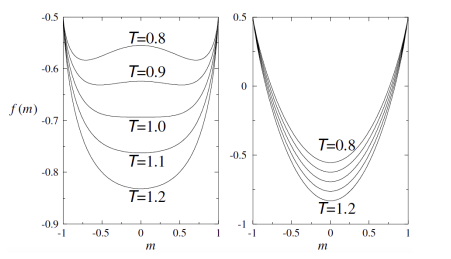
\includegraphics[width=0.8\textwidth]{img/constrainedfreeenergy.png}
    \caption{Comportamiento de la función de energía libre intensiva restringida $f(m)$ en función de la magnetización $m$ para diferentes valores de la temperatura $T$ y el parámetro de interacción $J$. Izquierda: $J=1$. Derecha: $J=-1$.}
    \label{fig:constrainedfreeenergy}
\end{figure}
\noindent
Ahora analizaremos las soluciones para $h\neq0$, pues antes habíamos impuesto dicha restricción para ver ciertas propiedades de la red, como por ejemplo que es par y por tanto simétrica, es decir, la elección entre el patrón y su inverso es equiprobable, y no venía afectada por un campo externo. \\

\noindent
Volviendo a la energía libre de la red, tenemos
\begin{equation*}
    f(m) = -\frac{Jm^2}{2} - hm + T \left[ \dfrac{1+m}{2} \log \left(\frac{1+m}{2}\right) + \frac{1-m}{2} \log \left(\frac{1-m}{2}\right) \right]
\end{equation*}
y la \tbf{ecuación de auto-consistencia generalizada} es
\begin{equation*}
    m^* = \tanh(\beta (Jm^* + h))
\end{equation*}
donde el campo externo $h$ rompe la simetría entre los dos estados de memoria, favoreciendo uno sobre el otro. Esto significa que la red tendrá una preferencia clara por recordar un patrón específico (por ejemplo, todas neuronas activas) en lugar de su inverso (todas inactivas). \\

\noindent
Es lógico que $m^*$ son los valores donde la derivada de $f(m)$ es cero, pero esto incluye tanto mínimos como máximos y puntos de inflexión. Nosotros nos interesaremos por los mínimos que son los estados estables de la red. Querremos ahora demostrar que $m^*$ es el valor esperado de la magnetización en el límite termodinámico (cuando $N\to \infty$), es decir
\begin{equation*}
    \lim_{N\to \infty} \omega_{N,J,h,\beta}(m_N(\sigma)) = m^*
\end{equation*}
donde $\omega_{N,J,h,\beta}$ representa el promedio estadístico de la magnetización bajo la medida de Boltzmann. El límite $\lim_{N\to \infty} \omega(m_N) = m^*$ te asegura que, en una red grande, no verás fluctuaciones locas: verás a la red comportándose de forma sólida y constante en este nivel de fidelidad $m^*$. \\

\noindent
Vamos a demostrar esto usando el \tbf{método del punto de silla}, para ellos necesitamos usar la siguiente identidad
\begin{equation*}
    e^{\frac{A}{2} O^2} = C' \int_{-\infty}^{\infty} e^{- \frac{x^2}{2A}  + Ox} dx
\end{equation*}
donde $C'$ es una constante de normalización. Usando esta identidad, podemos reescribir la función de partición $Z_{N,h,\beta}$ de la siguiente manera, donde usaremos $J=1$ para simplificar la notación
\begin{align*}
    Z_{N,h,\beta} &= \sum_{\sigma} e^{-\beta \mathcal{H}_{N,h}(\sigma)} = \sum_{\sigma} \exp \left[ \frac{\beta }{2N} \left( \sum_i \sigma_i \right)^2 + \beta h \left( \sum_i \sigma_i \right) \right]=\\
    &\overset{(*)}{=}\sum_{\sigma}\exp\left[\beta h \left( \sum_i \sigma_i \right)\right]C' \int_{-\infty}^{+\infty} \exp \left[ -\frac{y^2}{2(\beta / N)} + y \sum_i \sigma_i \right] \ dy =\\
    &\overset{(**)}{=}\sum_{\sigma} \exp\left[\beta h \left( \sum_i \sigma_i \right)\right] C 
    \int_{-\infty}^{+\infty} \exp \left[ - \frac{N \beta x^2}{2} + \beta x \sum_i \sigma_i \right] dx=\\
    &= C \int_{-\infty}^{+\infty}  \sum_{\sigma} \exp \left[ -N \beta \frac{x^2}{2} + \beta (h + x) \sum_i \sigma_i \right] dx= \\
    & = C \int_{-\infty}^{+\infty}  \exp\left(-N \beta \frac{x^2}{2}\right)\left[ \sum_{\sigma} \prod_{i=1}^{N} \exp\left(\beta (h + x) \sigma_i\right)\right] dx 
\end{align*}
donde en $(*)$ hemos aplicado la identidad anterior con $A = \beta / N$ y $O = \sum_{i} \sigma_i$, y en $(**)$ hemos hecho un cambio de variable $y=\beta x$. Resaltar que la expresión del Hamiltoniano usada es la siguiente
\begin{align*}
    \mathcal{H}_{N,J,h}(\sigma) = - \frac{NJ}{2} [m_N(\sigma)]^2 - hN m_N(\sigma)&=- \frac{N}{2} \left( \frac{1}{N} \sum_{i=1}^N \sigma_i \right)^2 - hN \left( \frac{1}{N} \sum_{i=1}^N \sigma_i \right)= \\
    &=- \left[ \frac{1}{2N} \left( \sum_{i=1}^N \sigma_i \right)^2 + h \sum_{i=1}^N \sigma_i \right]
\end{align*}

\noindent
Para seguir con el desarrollo anterior, vamos a ver que 
\begin{equation*}
    \sum_{\sigma} \dots = \sum_{\sigma_1 = \pm 1} \sum_{\sigma_2 = \pm 1} \dots \sum_{\sigma_N = \pm 1} \dots
\end{equation*}
donde lo que hacemos en la primera sumatoria es recorrer todas las posibles configuraciones de la red, y en las siguientes sumatorias recorremos cada neurona individualmente, dandole a la primera neurona el valor $+1$ y luego $-1$, y así sucesivamente con todas las neuronas, mientras que cuando avanzamos en la sumatoria de la primera neurona, las demás permanecen fijas. \\

\noindent
Veámos esta idea un poco más al detalle, pues lo que estamos haciendo es recorrer el estado individual de cada neurona por separado.
\begin{itemize}
    \item $\sum_{\sigma_1 = \pm 1}$: Esto significa "mira la neurona 1; primero ponla en $+1$ y luego en $-1$".
    \item $\sum_{\sigma_2 = \pm 1}$:Mientras la neurona 1 está fija, haz lo mismo con la neurona 2.
    \item Al poner todos estos sumatorios juntos, lo que haces es recorrer de forma sistemática todas las combinaciones posibles de los $N$ elementos.
\end{itemize} 
De esta manera, recorremos todas las configuraciones posibles de la red, y tenemos
\begin{align*}
    \sum_{\sigma} \prod_{i=1}^{N} \exp\left(\beta (h + x) \sigma_i\right)&=\sum_{\sigma_1 = \pm 1} \sum_{\sigma_2 = \pm 1} \dots \sum_{\sigma_N = \pm 1} \left[ e^{\beta(h+x)\sigma_1} \cdot e^{\beta(h+x)\sigma_2} \cdot \dots \cdot e^{\beta(h+x)\sigma_N} \right] = \\
    &= \left( \sum_{\sigma_1 = \pm 1} e^{\beta(h+x)\sigma_1} \right) \cdot \left( \sum_{\sigma_2 = \pm 1} e^{\beta(h+x)\sigma_2} \right) \dots \left( \sum_{\sigma_N = \pm 1} e^{\beta(h+x)\sigma_N} \right) =\\
    &\overset{(*)}{=}[2 \cosh(\beta(h+x))]^N
\end{align*}
donde en $(*)$ hemos usado que cada sumatorio es idéntico, y se calcula fácilmente como
\begin{equation*}
    \sum_{\sigma_i = \pm 1} e^{\beta(h+x)\sigma_i} = e^{\beta(h+x)} + e^{-\beta(h+x)} = 2 \cosh(\beta(h+x))
\end{equation*}

\noindent
Siguiendo con el desarrollo de $Z_{N,h,\beta}$, tenemos
\begin{align*}
    Z_{N,h,\beta} &= C \int_{-\infty}^{+\infty}  \exp \left[ -N \left( \beta \frac{x^2}{2} - \log 2 \cosh(\beta(h + x)) \right) \right] dx=C \int_{-\infty}^{+\infty} \exp(-N\phi(x)) \ dx \approx\\
    &\overset{(*)}{\approx}C \exp(-N\phi(x^*))
\end{align*}
donde en $(*)$ hemos aplicado el \tbf{método del punto de silla}, que nos dice que para $N$ grande, la integral está dominada por el valor mínimo de la función $\phi(x)$ dado por $x^*$, pues para el resto de puntos $x$ la exponencial decae muy rápido (queda como la función de dirac). Calculemos dicho mínimo
\begin{align*}
    \phi(x) &= \beta \frac{x^2}{2} - \log 2 \cosh(\beta(h + x)) \implies \phi'(x) = \beta x - \beta \dfrac{2\sinh(\beta(h+x))}{2\cosh(\beta(h+x))} = \\
    &= \beta x - \beta \tanh(\beta(h+x)) = 0 \implies x^* = \tanh(\beta(h+x^*))
\end{align*}
donde hemos usado que la derivada de $\cosh(x)$ es $\sinh(x)$. \\

\noindent
Por definición y propiedades de las observaciones térmicas, tenemos que
\begin{align*}
    \omega_N(m_N) &= -\dfrac{\partial f_N}{\partial h} = \dfrac{1}{N\beta} \dfrac{\partial \log Z_{N,h,\beta}}{\partial h}= \dfrac{1}{N\beta} \dfrac{\partial}{\partial h}\log \left(C \exp(-N\phi(x^*))\right) =\\
    &= \dfrac{1}{N\beta} \left[\dfrac{\partial }{\partial h} \log(C)- \dfrac{\partial}{\partial h} N\phi(x^*)\right]=-\dfrac{1}{\beta} \dfrac{\partial \phi(x^*)}{\partial h}
\end{align*}
por lo que calculemos ahora la derivada de $\phi(x^*)$ respecto a $h$
\begin{align*}
    \dfrac{\partial \phi(x^*)}{\partial h} &= \dfrac{\partial }{\partial h} \left[ \beta \frac{(x^*)^2}{2} - \log 2 \cosh(\beta(h + x^*)) \right] = \\
    &= \beta x^* \dfrac{\partial x^*}{\partial h} - \beta \dfrac{2\sinh(\beta(h+x^*))}{2\cosh(\beta(h+x^*))} \left(1 + \dfrac{\partial x^*}{\partial h} \right) = \\
    &= \beta x^* \dfrac{\partial x^*}{\partial h} - \beta \tanh(\beta(h+x^*)) \left(1 + \dfrac{\partial x^*}{\partial h} \right)=\\
    &=\dfrac{\partial x^*}{\partial h} \beta \left( x^* - \tanh(\beta(h+x^*)) \right) - \beta \tanh(\beta(h+x^*))=\\
    &\overset{(*)}{=}- \beta \tanh(\beta(h+x^*))
\end{align*}
donde hemos usado la regla de la cadena para derivar el segundo término, y en $(*)$ hemos usado que $x^*$ satisface la ecuación de auto-consistencia $x^* = \tanh(\beta(h+x^*))$, por lo que el primer término se anula. Finalmente, tenemos lo esperado
\begin{equation*}
    \omega(m)=\tanh(\beta(h+x^*))=x^*
\end{equation*}
que nos indica que el valor esperado de la magnetización en el límite termodinámico es igual a la solución de la ecuación de auto-consistencia. \\

\noindent
Aquí tenemos un resumen de lo que hemos logrado hasta ahora
\begin{itemize}
    \item El punto de mínima energía ($m^*$): representa el estado de mayor estabilidad termodinámica. Es el valor hacia el cual el sistema "quiere" ir naturalmente para minimizar su energía libre, pues es el punto mínimo de $f(m)$.
    \item El valor más esperado ($\omega(m) = x^*$): representa lo que realmente observarías si midieras la red. En el límite de muchas neuronas ($N \to \infty$), la probabilidad se concentra tanto en el punto de silla $x^*$ que cualquier fluctuación desaparece.
    \item La coincidencia ($\omega(m) = x^* = m^*$): al demostrar que estos valores son el mismo, estás probando que la realidad física (lo que mides) coincide con la estabilidad teórica (el mínimo de energía).
\end{itemize}
Ahora, sabiendo que la magentización converge a $x^*=m^*$, estudiaremos las soluciones de la ecuación de auto-consistencia para diferentes valores de la temperatura $T$ y el campo externo $h$, es decir, para que valores de $T$ y $h$ la red puede recordar patrones (tener $m^* \neq 0$) o no (tener $m^* = 0$). \\

\noindent
Primero, veamos el caso sin campo externo ($h=0$), para centrarnos en el ruido. En este caso, usaremos la aproximación de $\tanh(x)$ por la serie de Taylor alrededor de $x=0$, que es
\begin{equation*}
    \tanh(x) \approx x - \frac{x^3}{3} + O(x^5)
\end{equation*}
y aplicándola a la ecuación de auto-consistencia, tenemos
\begin{equation*}
    m = \tanh(\beta J m) \approx \beta Jm - \frac{(\beta Jm)^3}{3} + O(m^5)
\end{equation*}
donde tomamos $m^*=m$ por simplicidad y obviando los términos de orden superior, tenemos
\begin{equation*}
    m= \beta Jm - \frac{(\beta Jm)^3}{3} \implies m(J\beta - 1) = \frac{(\beta J)^3}{3} m^3 \implies m^2 = \frac{3(J\beta - 1)}{(\beta J)^3}
\end{equation*}
Llegados a este punto, tenemos dos casos
\begin{itemize}
    \item Si $J\beta < 1$ (es decir, $T > J$), entonces $m^2 < 0$, lo cual es imposible. Por lo tanto, la única solución física es $m = 0$. Esto significa que la red no puede recordar ningún patrón, ya que la magnetización es nula.
    \item Si $J\beta > 1$ (es decir, $T < J$), entonces $m^2 > 0$, y por lo tanto hay dos soluciones físicas posibles
    $$m = \pm\sqrt{\frac{3(J\beta - 1)}{(\beta J)^3}}$$
    Esto significa que la red puede recordar dos patrones (uno y su inverso), ya que la magnetización es diferente de cero.
\end{itemize}
Por tanto, hemos encontrado un punto crítico en la temperatura $T_c = \frac{1}{\beta_c}=J$, que separa dos fases distintas del sistema. Para que la fórmula sea más fácil de interpretar, aproximamos el término $(\beta J - 1)$ cerca de $T_c$
\begin{equation*}
    \beta J-1 = \frac{J}{T} - 1 = \frac{J - T}{T} \approx \frac{T_c - T}{T_c}
\end{equation*}
Sustituyendo esto en la fórmula de $m$ y asumiendo que cerca de $T_c$, $\beta J \approx 1$, entonces
\begin{equation*}
    m \approx \pm \sqrt{\frac{3(T_c - T)}{T_c}}
\end{equation*}
esta ecuación nos dice que la magnetización $m$ crece como la raíz cuadrada de la diferencia entre la temperatura crítica $T_c$ y la temperatura actual $T$, siempre que $T_c< T$. Al ser una raíz cuadrada, la pendiente en $T_c$ es infinita. Esto significa que en cuanto el ruido baja un milímetro por debajo del punto crítico, la red reacciona violentamente y empieza a formar un recuerdo muy rápido.  \\

\noindent
Finalmente, hemos encontrado los valores de temperatura $T$ que definen las dos fases del sistema
\begin{itemize}
    \item \tbf{Fase ordenada (memoria):} para $T < T_c$, la red puede recordar patrones, ya que la magnetización es diferente de cero ($m \neq 0$).
    \item \tbf{Fase desordenada (caos):} para $T > T_c$, la red no puede recordar ningún patrón, ya que la magnetización es nula ($m = 0$).
\end{itemize}
Este comportamiento es característico de una \tbf{transición de fase} en sistemas físicos, donde un cambio en un parámetro (en este caso, la temperatura) provoca un cambio abrupto en las propiedades del sistema (en este caso, la capacidad de memoria de la red neuronal).


\section{Phase transition}

\begin{definicion}
    En física, una \tbf{transición de fase} es cuando el agua se congela. En nuestra asignatura, ocurre cuando hay una singularidad (un "salto" o un cambio brusco) en la Energía Libre ($F$). Imagina que vas subiendo el ruido (temperatura $T$) en tu red. De repente, en un valor exacto de $T$, la red deja de reconocer el patrón. No lo hace poco a poco, sino que ``colapsa''. Ese punto exacto es la transición de fase. \\
\end{definicion}


\noindent
Para la clasificación de las transiciones de fase, usamos la \tbf{Clasificación de Ehrenfest}, que se basa en la continuidad de las derivadas de la energía libre ($F$):

\begin{itemize}
    \item \tbf{Primer orden}: hay una discontinuidad en la primera derivada de $F$. \underline{En la práctica}: la memoria desaparece de golpe (como el hielo fundiéndose).
    \item \tbf{Segundo orden (o continua)}: las primeras derivadas son continuas, pero las segundas fallan. \underline{En la práctica}: la capacidad de recordar va bajando suavemente hasta que llega a cero de forma nítida.
\end{itemize}

\noindent
El \tbf{parámetro de orden} es una variable que nos dice en qué fase estamos. En nuestro caso, es la magnetización ($m$). En nuestro caso el solapamiento ($m$), puede ser 
\begin{itemize}
    \item $m = 0$: Fase paramagnética (ruido total, no hay memoria).
    \item $m \neq 0$: Fase ferromagnética (la red recuerda, hay orden).
\end{itemize}

\subsubsection{Symmetry Breaking}
\noindent
En el modelo de Hopfield, si inviertes todas las neuronas ($\sigma_i \to -\sigma_i$), la energía es la misma. El sistema "no sabe" si prefiere el patrón o su inverso. Esto se llama \tbf{simetría}. \\

\begin{description}
    \item[En baja temperatura (Orden):] El sistema "elige" uno de los dos estados (el patrón o su inverso) y se queda ahí. Al elegir, rompe la simetría. \\
    \noindent
    Aplicación: Aprender es, esencialmente, romper la simetría del desorden para "caer" en un estado concreto (el recuerdo).
    \item[En alta temperatura (Caos):] La red salta tanto de un estado a otro que el promedio es cero. El sistema es simétrico. \\
\end{description}

\section{Ergodicity breaking}
\noindent
Cuando la temperatura (ruido) es alta ($T > T_c$), el sistema tiene tanta energía térmica que nada lo detiene. La red neuronal salta de un estado a otro sin parar. No se queda fija en ningún recuerdo, lo que significaría que es una red \tbf{ergódica}, por lo que decimos que el sistema ``explora todo el espacio $\Omega$''. \\

\noindent
Sin embargo, cuando la temperatura baja ($T < T_c$) (el sistema se \underline{enfría}), el sistema pierde energía térmica y se ``atasca'' en ciertos estados (recuerdos). La red ya no puede explorar todo el espacio de configuraciones posibles, sino que se queda atrapada en ciertos atractores. Esto se llama \tbf{ruptura de ergodicidad}. Lo que ocurre es que, el espacio de fases $\Omega$ se ``rompe'' en pedazos aislados (por ejemplo, $\Omega_+$ y $\Omega_-$), donde $\Omega_+$ podría representar el recuerdo de una ``Cara'', y $\Omega_-$ podría representar el recuerdo inverso (o un ``Gato''). \\

\noindent
En este sentido, decimos que el sistema se queda \tbf{confinado} en uno de estos subespacios, dependiendo de su estado inicial y de las fluctuaciones térmicas. La red ya no puede saltar libremente entre todos los estados posible (por ejemplo de $\Omega_+$ a $\Omega_-$), porque hay una barrera de energía gigante (proporcional al número de neuronas $N$). \\

\noindent
Para que esto sea ``memoria'', necesitamos comparar dos tiempos:
\begin{itemize}
    \item $\tau_0$ (\tbf{Tiempo de observación}): el tiempo que tardamos en usar la red.
    \item $\tau_{flip}$ (\tbf{Tiempo de salto}): el tiempo que tardaría la red en saltar de un recuerdo a otro por puro azar.
    \item \textbf{Ruptura de la Ergodicidad} ($\tau_0 \ll \tau_{flip}$): el salto es tan improbable (tardaría "tiempos astronómicos", más que la edad del universo) que, para nosotros, el sistema está en equilibrio local. ¡Esto es la memoria! La red se queda fija en el patrón que le hemos pedido recuperar.
\end{itemize}
Un punto a notar importante es que, en teoría, si esperasemos trillones de años, el sistema acabaría saltando de un valle a otro y recuperaría la ergodicidad. Sin embargo, en la práctica, como nosotros usamos la red neuronal durante unos segundos o minutos (un tiempo $\tau_0$ muy pequeño), para nosotros el sistema está en equilibrio local y no vemos esos saltos. Esta es la justificación matemática de por qué podemos decir que una red neuronal ha ``convergido'' a una solución, aunque técnicamente el universo siga evolucionando. \\

\noindent
¿Por qué es importante esto en el modelo de Hopfield? Si la red fuera siempre ergódica, tú le darías una imagen borrosa y ella empezaría a oscilar entre todos los patrones que conoce sin detenerse en ninguno. La ruptura de la ergodicidad es lo que permite que la red ``tome una decisión'' y se quede en un valle de energía (atractor).

\section{Hopfield model}
\noindent
El modelo de Hopfield es la evolución natural del modelo de Curie-Weiss (CW) que hemos estado analizando. Mientras que en el modelo CW las neuronas solo aprendían a ``ponerse todas de acuerdo'' (almacenando solo 1 bit de información), el modelo de Hopfield permite que la red actúe como una memoria asociativa capaz de almacenar y recuperar múltiples patrones complejos. \\


\noindent
La tarea principal de esta red es la reconstrucción de $P$ ``piezas de información''. Estas piezas son vectores binarios $\{\xi^\mu\}$ de longitud $N$. Imagina que cada vector $\xi^\mu$ es una imagen o un concepto (por ejemplo, una foto de un gato). La red debe ser capaz de ``recordar'' esa imagen completa incluso si solo le das una parte borrosa o con ruido. En lugar de tener solo dos valles en $+1$ y $-1$, el modelo de Hopfield diseña el paisaje para que haya un ``valle'' (mínimo de energía) en cada uno de los patrones $\xi^\mu$ que queremos recordar. \\

\noindent
En el modelo CW, las conexiones entre neuronas eran uniformes (todas las neuronas se influían igual), es decir, $J_{ij} = \frac{J}{N}$. En el modelo de Hopfield, las conexiones son específicas y se diseñan para almacenar los patrones deseados. La \tbf{regla de aprendizaje de Hebb} nos dice cómo ajustar estas conexiones de la siguiente manera
\begin{equation*}
    J_{ij} = \frac{1}{N} \sum_{\mu=1}^{P} \xi_i^\mu \xi_j^\mu
\end{equation*}
donde $\xi_i^\mu$ es el estado (activo o inactivo) de la neurona $i$ en el patrón $\mu$. Esta regla asegura que las neuronas que tienden a activarse juntas (en el mismo patrón) refuercen su conexión, mientras que las que no lo hacen debilitan su vínculo. Ahora el hamiltoniano del sistema es
\begin{equation*}
    \mathcal{H}_{N,\xi,h}(\sigma) = -\frac{1}{N} \sum_{i,j<i} \sum_\mu \xi_i^\mu \xi_j^\mu \sigma_i \sigma_j - \sum_i h_i \sigma_i 
\end{equation*}
donde $\sigma_i$ es el estado actual de la neurona $i$. \\

\noindent
Nos centraremos en estudiar como la red puede recuperar un patrón específico $\xi^\nu$ cuando se le presenta una versión ruidosa o incompleta del mismo, por lo que definiremos $h=0$, ya que queremos estudiar la capacidad de memoria pura de la red sin influencias externas, pues estas pueden ser beneficiosas para la clasificación, y es eso justo lo que no queremos, intentando estudiar solo como reacciona la red en sí. \\

\subsection{Low-load regime}
\noindent
En esta sección nos centraremos en el \tbf{régimen de baja carga} (low-load), donde el número de patrones almacenados $P$ es mucho menor que el número de neuronas $N$ (es decir, $\alpha=P/N \to 0$ cuando $N \to \infty$). En este régimen, la red puede manejar múltiples patrones sin que interfieran entre sí, lo que facilita el análisis. \\


\begin{definicion}
    Consider the Hopfield model with $N$ neurons $\sigma_i$, $i \in \{1, \ldots, N\}$ and $P$ patterns $\xi^\mu$, $\mu \in \{1, \ldots, P\}$, the \tbf{Hamiltonian} is defined as
    \begin{align*}
        H_{N,\xi}(\sigma) &= -\frac{1}{N} \sum_{i,j<i} \sum_{\mu=1}^{P} \xi_i^\mu \xi_j^\mu \sigma_i \sigma_j=-\dfrac{1}{2N} \sum_{i,j,\mu} \xi_i^\mu \xi_j^\mu \sigma_i \sigma_j + \dfrac{1}{2N} \sum_{i,\mu} \left(\xi_i^\mu\right)^2\sigma_i^2=\\
        &= -\dfrac{1}{2N} \sum_{i,j,\mu} \xi_i^\mu \xi_j^\mu \sigma_i \sigma_j +\dfrac{P}{2}
    \end{align*}
    Definimos las siguientes funciones 
    \begin{itemize}
        \item the \tbf{(pattern realization dependent) partition function} as
        \begin{equation*}
            Z_{N,\beta,\xi} = \sum_{\sigma} e^{-\beta H_{N,\xi}(\sigma)}
        \end{equation*}
        \item the \tbf{Boltzmann factor} as
        \begin{equation*}
            B_{N,\beta,\xi}(\sigma) = e^{-\beta H_{N,\xi}(\sigma)}
        \end{equation*}
        \item the \tbf{Boltzmann-Gibbs average} as
        \begin{equation*}
            \omega_{N,\xi}(F) = \frac{\sum_{\sigma} F(\sigma) B_{N,\beta,\xi}(\sigma)}{\sum_{\sigma} B_{N,\beta,\xi}(\sigma)}
        \end{equation*}
        for any arbitrary function $F(\sigma)$ of the spins.
        \item the \tbf{quenched statistical pressure} as
        \begin{equation*}
            A_{N,\beta} = -\beta f_{N,\beta}^Q, \quad f_{N,\beta}^Q = -\frac{1}{\beta N} \mathbb{E} \log Z_{N,\beta,\xi}
        \end{equation*}
        where $f_{N,\beta}^Q= - \frac{1}{\beta N} \mathbb{E} \log Z_{N,\beta,\xi}$ is the \tbf{(quenched) free energy}. \\
    \end{itemize}
\end{definicion}
\noindent
Para resolver el modelo de Hopfield, lo que buscamos es querer demostrar que la red es capaz de recordar los patrones almacenados $\{\xi^\mu\}$, es decir, que la red puede converger a uno de estos patrones cuando se le presenta una versión ruidosa o incompleta del mismo. Para ello, debemos determinar el valor de los \tbf{solapamientos} u \tbf{order parameters} de  $m_\mu$, que miden la similitud entre el estado actual de la red $\sigma$ y cada patrón almacenado $\xi^\mu$. Estos solapamientos se definen como
\begin{equation*}
    m_\mu(\sigma) = \frac{1}{N} \sum_{i=1}^{N} \xi_i^\mu \sigma_i
\end{equation*}
donde $m_\mu$ toma valores entre $-1$ y $+1$. Un valor de $m_\mu$ cercano a $+1$ indica que la red está en un estado muy similar al patrón $\xi^\mu$, mientras que un valor cercano a $-1$ indica que la red está en el patrón inverso. Un valor cercano a $0$ significa que la red no tiene correlación con ese patrón. \\

\noindent
The main interest of this section and of the two following ones (for which the same
definitions hold) is to find the expression of the free energy in the thermodynamic limit
$f_\beta^Q = \lim_{N \to \infty} f_{N,\beta}^Q$ in terms of the order parameters, both in the low and high storage regimes.

\subsubsection{Saddle Point Method}
\noindent
Antes de proceder con el desarrollo del modelo de Hopfield, repasemos brevemente el \tbf{método del punto de silla} (saddle point method), que ya hemos usado en la sección anterior. Este método es una técnica matemática utilizada para aproximar integrales de la forma
\begin{equation*}
    I(N) = \int e^{-N \phi(x)} \ dx
\end{equation*}
cuando $N$ es grande. La idea principal es que, para valores grandes de $N$, la integral está dominada por las regiones donde la función $\phi(x)$ es mínima, ya que la exponencial decae rápidamente en otras regiones. \\

\noindent
También, es importante destacar esta igualdad que usaremos en el desarrollo posterior procedente de la delta de Dirac
\begin{align*}
    \int_{-\infty}^{+\infty} f(x) \delta(x - a) \ dx = f(a) \implies \int_{-\infty}^{+\infty} g(m_{\mu})\delta\left(m_{\mu} - \dfrac{1}{N}\sum_{i} \xi_i^{\mu} \sigma_i\right) \ dm_{\mu} = 1
\end{align*}
donde $g(x)=1$. Aplicando esto a todos los patrones $\mu \in \{1, \ldots, P\}$, tenemos
\begin{equation*}
    \prod_{\mu=1}^{P} \int_{-\infty}^{+\infty} \delta\left(m_{\mu} - \dfrac{1}{N}\sum_{i} \xi_i^{\mu} \sigma_i\right) \ dm_{\mu} = 1
\end{equation*}
Usando esta identidad, y el siguiente desarrollo
\begin{align*}
    \sum_{i,j} \xi_i^\mu \xi_j^\mu \sigma_i \sigma_j &= \left( \sum_{i} \xi_i^\mu \sigma_i \right)^2 = N^2 m_\mu^2\implies \frac{\beta}{2N} \sum_{\mu=1}^P \left( \sum_{i} \xi_i^\mu \sigma_i \right)^2= \frac{\beta N}{2} \sum_{\mu=1}^P m_\mu^2
\end{align*}
podemos reescribir la función de partición del modelo de Hopfield como
\begin{align*}
    Z_{N,\beta,\xi} &= \sum_{\sigma} \exp \left[ \frac{\beta}{2N} \sum_{i,j,\mu} \xi_i^\mu \xi_j^\mu \sigma_i \sigma_j  \right]= \sum_{\sigma} \int \exp\left(\dfrac{\beta N}{2} \sum_{\mu=1}^P m_\mu^2\right) \prod_{\mu=1}^{P} \left[\delta\left(m_{\mu} - \dfrac{1}{N}\sum_{i} \xi_i^{\mu} \sigma_i\right) \ dm_{\mu}\right]
\end{align*}
donde hemos obviado el término constante $\exp\left(-\beta P/2\right)$, ya que no afecta a las observables térmicas, cuando $N$ es grande. Ahora buscaremos aplicar la definición formal de la delta de Dirac
\begin{align*}
    \delta(x) = \frac{1}{2\pi} \int_{-\infty}^{\infty} e^{ikx} dk &\implies \delta(x-y)= \frac{1}{2\pi} \int_{-\infty}^{\infty} e^{ik(x-y)} dk \implies \\
    &\implies \delta\left(m_{\mu}-\dfrac{1}{N}\sum_{i} \xi_i^{\mu} \sigma_i\right)=\dfrac{1}{2\pi}\int_{-\infty}^{+\infty}\exp\left(ik\left(m_{\mu}-\dfrac{1}{N}\sum_{i} \xi_i^{\mu} \sigma_i\right)\right) dk
\end{align*}
además de hacer un cambio de variable $k=N\bar{m_{\mu}}$. Veamos todos los pasos al aplicar estos conceptos
\begin{align*}
    Z_{N,\beta,\xi}&=\sum_{\sigma}\int \exp\left(\dfrac{\beta N}{2} \sum_{\mu=1}^P m_\mu^2\right) \prod_{\mu=1}^{P} \left[\exp\left(ik_{\mu}\left(m_{\mu}-\dfrac{1}{N}\sum_{i} \xi_i^{\mu} \sigma_i\right)\right) \ \dfrac{dm_{\mu}dk_{\mu}}{2\pi}\right]=\\
    &\overset{(*)}{=}\sum_{\sigma}\int \exp\left(\dfrac{\beta N}{2} \sum_{\mu=1}^P m_\mu^2\right) \prod_{\mu=1}^{P} \left[\exp\left(iN\bar{m_{\mu}}\left(m_{\mu}-\dfrac{1}{N}\sum_{i} \xi_i^{\mu} \sigma_i\right)\right) \ \dfrac{Ndm_{\mu}d\bar{m_{\mu}}}{2\pi}\right]=\\
    &=\sum_{\sigma}\int \exp\left(\dfrac{\beta N}{2} \sum_{\mu=1}^P m_\mu^2\right) \prod_{\mu=1}^{P} \left[\dfrac{Ndm_{\mu}d\bar{m_{\mu}}}{2\pi}\right] \exp\left[iN \sum_{\mu}\bar{m_{\mu}}\left(m_{\mu}-\dfrac{1}{N}\sum_i \xi_i^{\mu}\sigma_i\right)\right]=\\
    &=\sum_{\sigma}\int \prod_{\mu=1}^{P} \left[\dfrac{Ndm_{\mu}d\bar{m_{\mu}}}{2\pi}\right] \exp\left(iN\sum_{\mu}\bar{m_{\mu}}m_{\mu}- i \sum_{i,\mu}\bar{m_{\mu}}\xi_i^{\mu}\sigma_i + \dfrac{\beta N}{2} \sum_{\mu} m_\mu^2 \right)
\end{align*}
donde en $(*)$ hemos hecho el cambio de variable $k_{\mu}=N\bar{m_{\mu}}$. Ahora volveremos a usar una idea similar a la que usamos en la sección anterior, es decir, que
\begin{align*}
    \sum_{\sigma} \exp\left(-i \sum_{i,\mu}\bar{m_{\mu}}\xi_i^{\mu}\sigma_i\right) &= \prod_{i=1}^{N} \sum_{\sigma_i = \pm 1} \exp\left(-i \sigma_i \sum_{\mu} \bar{m_{\mu}} \xi_i^{\mu}\right) = \\
    &\overset{(*)}{=}\prod_{i=1}^{N} 2\cos\left(\sum_{\mu} \bar{m_{\mu}} \xi_i^{\mu}\right) =\exp\left(\ln\left[ \prod_{i=1}^{N} 2\cos\left(\sum_{\mu} \bar{m_{\mu}} \xi_i^{\mu}\right) \right]\right) = \\
    &=\exp\left( \sum_{i=1}^N \ln \left[ 2 \cos\left( \sum_{\mu} \bar{m}_{\mu} \xi_i^{\mu} \right) \right] \right)
\end{align*}
o más desarrollado la primera parte
\begin{align*}
    \sum_{\sigma} \exp\left(-i \sum_{i,\mu}\bar{m_{\mu}}\xi_i^{\mu}\sigma_i\right) &= \sum_{\sigma} \exp\left(-i \sum_i \sigma_i \sum_{\mu} \bar{m_{\mu}} \xi_i^{\mu}\right)=\\
    &=\sum_{\sigma} \exp\left( -i\sigma_1 \sum_{\mu} \bar{m_{\mu}} \xi_1^{\mu} \right) \ldots \exp\left( -i\sigma_N \sum_{\mu} \bar{m_{\mu}} \xi_N^{\mu} \right)=\\
    &=\sum_{\sigma_1=\pm 1} \exp\left( -i\sigma_1 \sum_{\mu} \bar{m_{\mu}} \xi_1^{\mu} \right) \ldots \sum_{\sigma_N=\pm 1} \exp\left( -i\sigma_N \sum_{\mu} \bar{m_{\mu}} \xi_N^{\mu} \right)=\\
    &\overset{(*)}{=}2\cos\left( \sum_{\mu} \bar{m_{\mu}} \xi_1^{\mu} \right) \ldots  2\cos\left( \sum_{\mu} \bar{m_{\mu}} \xi_N^{\mu} \right)=\\
    &= \prod_{i=1}^{N} 2\cos\left(\sum_{\mu} \bar{m_{\mu}} \xi_i^{\mu}\right)
\end{align*}
donde en $(*)$ hemos usado que $e^{ix} + e^{-ix} = 2 \cos(x)$. Tenemos ahora la función de partición como
\begin{equation}
    Z_{N,\beta,\xi} = \int \prod_{\mu=1}^{P} \left[\dfrac{Ndm_{\mu}d\bar{m_{\mu}}}{2\pi}\right] \exp\left( iN \sum_{\mu} \bar{m_{\mu}} m_{\mu} + \sum_i\ln \left[ 2 \cos\left( \sum_{\mu} \bar{m}_{\mu} \xi_i^{\mu} \right) \right] + \dfrac{\beta N}{2} \sum_{\mu} m_\mu^2 \right) \quad \label{eq:particion_hopfield}
\end{equation}
Cuando $N$ es grande, podemos aplicar el \tbf{método del punto de silla} para aproximar la integral, donde buscaremos el mínimo primero para $m_{\mu}$ y luego para $\bar{m_{\mu}}$. Primero nos centraremos en minimizar respecto a $m_{\mu}$ , por lo que derivaremos el exponente respecto a $m_{\mu}$ (debemos fijar $\mu$ pues el resto de $m_{\nu}$ son distintas para $\mu\neq \nu$) y lo igualaremos a cero
\begin{align*}
    \dfrac{\partial}{\partial m_{\mu}} \left( iN \sum_{\mu} \bar{m_{\mu}} m_{\mu} + \sum_i\ln \left[ 2 \cos\left( \sum_{\mu} \bar{m}_{\mu} \xi_i^{\mu} \right) \right] + \dfrac{\beta N}{2} \sum_{\mu} m_\mu^2 \right) &= iN \bar{m_{\mu}} + \beta N m_{\mu} = 0 \implies \\
    & \implies \bar{m_{\mu}} = \dfrac{-\beta m_{\mu}}{i}= i \beta m_{\mu}
\end{align*}
notar que aunque hemos derivado respecto a $m_{\mu}$, hemos despejado para $\bar{m_{\mu}}$, pues buscamos tener la expresión de la función de partición en función de los ordenes de parámetro $m_{\mu}$. Ahora, sustituyendo este valor de $\bar{m_{\mu}}$ en la función de partición, y aplicando el método del punto de silla (donde eliminamos por tanto las integrales respecto a $\bar{m_{\mu}}$), tenemos

\begin{equation*}
    Z_{N,\beta,\xi} \underset{N \to \infty}{\sim} \int \left( \prod_{\mu} dm_\mu \right) \exp \left( -\frac{\beta N}{2} \sum_{\mu=1}^P m_\mu^2 + \sum_{i} \ln \left[ 2 \cosh \left( \beta \sum_{\mu} m_\mu \xi_i^\mu \right) \right] \right)
\end{equation*}
debemos destacar que hemos usado que $\cos(ix) = \cosh(x)$.\\

\noindent
Hemos obtenido una expresión de la función de partición en términos de los órdenes de parámetro $m_{\mu}$, pero realmente queremos poder quitar la integral, por lo que para ello aplicaremos el método del punto de silla a la vez, tanto para $m_{\mu}$ como para $\bar{m_{\mu}}$. Por tanto, derivamos el exponente que teníamos en \ref{eq:particion_hopfield} respecto a $\bar{m_{\mu}}$ y lo igualamos a cero 
\begin{align*}
    iN m_{\mu} + \sum_i \dfrac{-\sin\left( \sum_{\mu} \bar{m_{\mu}} \xi_i^{\mu} \right)}{\cos\left( \sum_{\mu} \bar{m_{\mu}} \xi_i^{\mu} \right)} \xi_i^{\mu} = 0 &\implies iN m_{\mu} - \sum_i\xi_i^{\mu} \tan\left( \sum_{\mu} \bar{m_{\mu}} \xi_i^{\mu} \right)  = 0 \implies \\
    &\implies m_{\mu} = -\dfrac{i}{N} \sum_j \xi_i^{\mu} \tan\left( \sum_{\nu} \bar{m_{\nu}} \xi_j^{\nu} \right) 
\end{align*}
Ahora tomando el mínimo $m_{\mu}^*$ para este valor de $m_{\mu}$ y el valor de $\bar{m_{\mu}}$ que habíamos obtenido antes, tenemos el sistema de ecuaciones
\begin{equation*}
    \begin{cases}
        \bar{m_{\mu}} = i \beta m_{\mu}^* \\
        m_{\mu} =m_{\mu}^*= -\dfrac{i}{N} \sum\limits_j \xi_i^{\mu} \tan\left( i \beta \sum\limits_{\mu} m_{\mu}^* \xi_j^{\mu} \right)
    \end{cases} \implies \quad m_{\mu}^* = \dfrac{1}{N} \sum_j \xi_i^{\mu} \tanh\left( \beta \sum_{\nu} m_{\nu} \xi_j^{\nu} \right)
\end{equation*}
donde hemos usado que $\tan(ix) = i \tanh(x)$. Finalmente, aplicamos el método del punto de silla en la función de partición, sustituyendo el valor $m_{\mu}^*$ en la expresión, obteniendo
\begin{equation*}
    Z_{N,\beta,\xi} \underset{N \to \infty}{\sim} \left(\dfrac{N}{2\pi}\right)^{\frac{P}{2}}\exp \left( -\frac{\beta N}{2} \sum_{\mu=1}^P (m_{\mu}^*)^2 + \sum_{i} \ln \left[ 2 \cosh \left( \beta \sum_{\mu} m_{\mu}^* \xi_i^\mu \right) \right] \right)
\end{equation*}
donde la parte del productorio $\left(\frac{N}{2\pi}\right)^{\frac{P}{2}}$ es irrelevante en el límite termodinámico, pues al calcular la free energy, esta parte se anula al dividir por $N$ y hacer $N \to \infty$. Entonces, the (quenched) free energy in the thermodynamic limit is
\begin{align*}
    f_{\beta}^Q &= \lim_{N \to \infty} f_{N,\beta}^Q = \lim_{N\to \infty}\left[-\frac{1}{\beta N} \mathbb{E} \log Z_{N,\beta,\xi} \right]= \\
    &=\lim_{N \to \infty} \mathbb{E}_{\xi} \left[ \frac{1}{2} \sum_{\mu=1}^P (m_{\mu}^*)^2 - \frac{1}{\beta N} \sum_{i=1}^N \ln \left( 2 \cosh \left( \beta \sum_{\mu=1}^P m_{\mu}^* \xi_i^\mu \right) \right) \right]=\\
    &= \min_{m} \left[ \dfrac{1}{2} \sum_{\mu=1}^P m_{\mu}^2 - \dfrac{1}{\beta} \mathbb{E} \log 2 \cosh\left( \beta \sum_{\mu=1}^P m_{\mu} \xi^{\mu} \right) \right]
\end{align*}
donde lo que hemos aplicado es definir la variable aleatoria $X_i$ para cada neurona $i$ como
\begin{equation*}
    X_i = \ln \left( 2 \cosh \left( \beta \sum_{\mu=1}^P m_{\mu}^* \xi_i^\mu \right) \right)
\end{equation*}
que por la ley de los grandes números (cumple las hipótesis trivialmente), cuando $N \to \infty$, tenemos que
\begin{equation*}
    \frac{1}{N} \sum_{i=1}^N X_i \underset{N \to \infty}{\to} \mathbb{E}[X] = \mathbb{E}_{\xi} \left[ \ln \left( 2 \cosh \left( \beta \sum_{\mu=1}^P m_{\mu}^* \xi^{\mu} \right) \right) \right] \quad \text{ c.s.}
\end{equation*}
Ahora bien, necesitamos ver como calcular la esperenza respecto a los patrones $\xi$. En nuestro caso, el ``experimento'' es elegir los $P$ bits de una neurona al azar. Definimos un vector aleatorio \mbox{$\xi = (\xi^1, \xi^2, \dots, \xi^P)$} que representa los bits de una neurona genérica (puede tomar $\pm 1$ con probabilidad $1/2$ cada uno). Entonces, la esperanza que necesitamos calcular es
\begin{equation*}
    \mathbb{E}[g(\xi)] = \sum_{\text{todas las configuraciones } \xi} P(\xi) \cdot g(\xi) 
\end{equation*}
donde sustituyendo nuestra $P(\xi) = 1/2^P$ y expandiendo la suma para cada componente del vector, obtenemos la siguiente ecuación
\begin{equation*}
    \mathbb{E} [g(\xi)] = \frac{1}{2^P} \sum_{\xi^1=\pm 1} \sum_{\xi^2=\pm 1} \dots \sum_{\xi^P=\pm 1} g(\xi^1, \xi^2, \dots, \xi^P)
\end{equation*}
y por tanto sabemos como calcular la esperanza respecto a los patrones $\xi$. \\

\noindent
Ahora para demostrar el siguiente enunciado, debemos recordar que los valores de $m_{\mu}$ que minimizan la quenched free-energy son los obtenidos al derivar la quenched free-energy respecto a $m_{\mu}$ y igualar a cero
\begin{align*}
    \frac{\partial f}{\partial m_\mu} &= \frac{\partial}{\partial m_\mu} \left[ \frac{1}{2} \sum_{\nu=1}^P m_\nu^2 - \frac{1}{\beta} \mathbb{E} \ln \left( 2 \cosh \left( \beta \sum_{\nu=1}^P m_\nu \xi^\nu \right) \right) \right] = \\
    & =m_{\mu}-\frac{1}{\beta} \mathbb{E} \left[ \tanh \left( \beta \sum m_\nu \xi^\nu \right) \cdot \beta \xi^\mu \right] = 0 \\
    & \implies m_{\mu} = \mathbb{E}_{\xi} \left[ \xi^{\mu} \tanh \left( \beta \sum_{\nu=1}^P m_{\nu} \xi^{\nu} \right) \right]
\end{align*}
\begin{teo}
    The quenched free-energy of the Hopfield model in the thermodynamic limit of
    the low-storage regime is
    \begin{equation*}
        f_{\beta}^Q = \min_{m} \left[ \dfrac{1}{2} \sum_{\mu=1}^P m_{\mu}^2 - \dfrac{1}{\beta} \mathbb{E} \log 2 \cosh\left( \beta \sum_{\mu=1}^P m_{\mu} \xi^{\mu} \right) \right]
    \end{equation*}
    where the Mattis magnetizations satisfy the \tbf{self-consistency equations}
    \begin{equation*}
        m_{\mu}^* = \mathbb{E}_{\xi} \left[ \xi^{\mu} \tanh \left( \beta \sum_{\nu=1}^P m_{\nu}^* \xi^{\nu} \right) \right]
    \end{equation*}
    at the equilibrium states.
\end{teo}
\noindent
Ahora veremos ciertos comentarios muy importantes respecto a la solución obtenida.
\begin{description}
    \item[Notación Vectorial y el Estado de Equilibrio.] Usando una notación vectorial más compacta, podemos escribir la energía libre y las ecuaciones de auto-consistencia como
    \begin{align*}
        f_{\beta} &= \dfrac{1}{2} \mathbf{m}^2 - \dfrac{1}{\beta} \mathbb{E} \log 2 \cosh(\beta \mathbf{m} \cdot \mathbf{\xi}) \quad \text{ tal que } \mathbf{m} = \mathbb{E} \mathbf{\xi} \tanh(\beta \mathbf{m} \cdot \mathbf{\xi})
    \end{align*}
    donde $\mathbf{m}$ es la \tbf{ecuación de auto-consistencia}, que indica que el estado de equilibrio de la red (su magnetización) debe ser igual al promedio de la respuesta de las neuronas ante el campo creado por los patrones.
    \item[El Límite de Recuperación Pura (Curie-Weiss).] Si suponemos que la red solo intenta recuperar el patrón 1 ($m_1 \neq 0$ y los demás $m_\mu = 0$), ocurre algo muy elegante: La ecuación se reduce a
    \begin{equation*}
        m_1 = \mathbb{E} [\xi^1 \tanh(\beta m_1 \xi^1)]
    \end{equation*}
    como la función $\tanh$ es impar, $\tanh(\beta m_1 \xi^1) = \xi^1 \tanh(\beta m_1)$, y $\xi^1 = \pm 1$, entonces al multiplicar por la $\xi^1$ de fuera, obtenemos $(\xi^1)^2 = 1$, lo que nos da lo siguiente
    \begin{equation*}
        m_1 = \tanh(\beta m_1)
    \end{equation*}
    Esta es la \tbf{Ley de Curie-Weiss} que describe a los imanes. Esto demuestra que, si solo hay un patrón, la red de Hopfield se comporta exactamente como un material ferromagnético donde los ``espines'' se alinean para formar el recuerdo.
    \item[Simetría de las Variables Auxiliares.] Al derivar respecto a $m_\mu$ y $\bar{m}_\mu$ simultáneamente, realmente no se calculó la ``energía libre restringida'' (que es más difícil), pero que matemáticamente no importa: los puntos de equilibrio (mínimos) son los mismos.
\end{description}

\subsubsection{Analysis of the self-consistency equation}
\noindent
El análisis de la ecuación de auto-consistencia
\begin{equation*}
    m_{\mu} = \mathbb{E}_{\xi} \left[ \xi^{\mu} \tanh \left( \beta \sum_{\nu=1}^P m_{\nu} \xi^{\nu} \right) \right]
\end{equation*}
muestra que existe un umbral $\beta_c = 1$ tal que
\begin{itemize}
    \item si $\beta < \beta_c$, $m = 0$ es la única solución;
    \item si $\beta > \beta_c$, resulta $m \neq 0$ y hay muchas soluciones admisibles.
\end{itemize}
Para probar esto, sabiendo donde esta el umbral $\beta_c$, tomaremos una pequeña desviación $\epsilon=\beta-1\ll1$, cerca de este punto, los valores de $m_{\mu}$ son muy pequeños (cuanto más crezca $\beta$ respecto a $\beta_c$ más irá creciendo $m_{\mu}$), lo que nos permite usar la aproximación de Taylor para la tangente hiperbólica

\begin{equation*}
    \tanh(x) = x - \frac{1}{3}x^3 + \frac{2}{15}x^5 - \dots
\end{equation*}
Sustituimos esto en nuestra ecuación original
\begin{equation*}
    m_{\mu} \approx \mathbb{E}_{\xi} \left[ \xi^{\mu} \left( \beta \sum_{\nu} m_{\nu} \xi^{\nu} - \frac{1}{3} \left( \beta \sum_{\nu} m_{\nu} \xi^{\nu} \right)^3 \right) \right]
\end{equation*}
Debemos resolver la esperanza término a término, recordando que $\mathbb{E}[\xi^{\mu}\xi^{\nu}] = \delta_{\mu\nu}$ (son independientes) y que $(\xi^{\mu})^2 = 1$.
\begin{itemize}
    \item \textbf{Término Lineal:}
    \begin{equation*}
        \mathbb{E} [ \xi^{\mu} \beta \sum_{\nu} m_{\nu} \xi^{\nu} ] = \beta \sum_{\nu} m_{\nu} \mathbb{E}[\xi^{\mu} \xi^{\nu}] = \beta m_{\mu}
    \end{equation*}
    \item \textbf{Término Cúbico:} Sea $X = \sum_{\nu} m_{\nu} \xi^{\nu}$. El término es $-\frac{1}{3}\beta^3 \mathbb{E}[\xi^{\mu} X^3]$. Al expandir $X^3$ y promediar sobre el ruido, los únicos términos que sobreviven son aquellos donde los índices de $\xi$ se emparejan. El resultado de esta combinatoria es:
    \begin{align*}
        \mathbb{E}[\xi^{\mu} X^3] &= \sum_{\alpha, \gamma, \delta} m_{\alpha} m_{\gamma} m_{\delta} \mathbb{E}[\xi^{\mu} \xi^{\alpha} \xi^{\gamma} \xi^{\delta}]=  m_{\mu}^3 + 3 \sum_{\nu \neq \mu} m_{\mu} m_{\nu}^2= \\
        &= m_{\mu}^3 + 3 \left( \sum_{\nu=1}^P m_{\mu} m_{\nu}^2 - m_{\mu} m_{\mu}^2 \right)= m_{\mu}^3 + 3 m_{\mu} \left( \sum_{\nu=1}^P m_{\nu}^2 \right) - 3 m_{\mu}^3=\\
        &= 3 m_{\mu} \left( \sum_{\nu=1}^P m_{\nu}^2 \right) - 2 m_{\mu}^3=3 m_{\mu} \mathbf{m}^2 - 2 m_{\mu}^3
    \end{align*}
    donde hemos usado que
    \begin{align*}
        \bb{E}[\xi^{\mu}]&=P(\xi^{\mu}=+1)(\xi^{\mu}=+1)+P(\xi^{\mu}=-1)(\xi^{\mu}=-1)=\frac{1}{2}(+1)+\frac{1}{2}(-1)=0 \\
        \bb{E}[(\xi^{\mu})^2]&= P(\xi^{\mu}=+1)(\xi^{\mu}=+1)^2+P(\xi^{\mu}=-1)(\xi^{\mu}=-1)^2=\frac{1}{2}(+1)^2+\frac{1}{2}(-1)^2=1
    \end{align*}
    de manera que 
    \begin{itemize}
        \item \tbf{Regla de imparidad}: si algún índice $\xi$ aparece un número impar de veces (como 1 o 3), el promedio es $0$.
        \item \tbf{Regla de paridad}: si todos los índices aparecen un número par de veces (como 2 o 4), el promedio es $1$ (porque $(\xi)^2 = 1$ y $(\xi)^4 = 1$).
    \end{itemize}
\end{itemize}
Agrupando los resultados, tenemos
\begin{align*}
    m_{\mu} &\approx \beta m_{\mu} - \frac{1}{3}\beta^3 (3m_{\mu} \mathbf{m}^2 - 2m_{\mu}^3)= m_{\mu}(1+\epsilon)- \dfrac{(1+\epsilon)^3}{3}(3m_{\mu} \mathbf{m}^2 - 2m_{\mu}^3)\implies\\
    &\implies m_{\mu}-m_{\mu}=m_{\mu}\epsilon - (1+\epsilon)^3 m_{\mu} \mathbf{m}^2 + \dfrac{2}{3}(1+\epsilon)^3 m_{\mu}^3 \implies \\
    &\implies m_{\mu} \left[ \epsilon - (1+\epsilon)^3 \mathbf{m}^2 + \dfrac{2}{3}(1+\epsilon)^3 m_{\mu}^2 \right] = 0
\end{align*}
entonces tenemos dos posibilidades:
\begin{itemize}
    \item Si $m_{\mu} = 0$ para todo $\mu$, tenemos la solución trivial (estado desordenado).
    \item Si $m_{\mu} \neq 0$ para algún $\mu$, entonces el término entre corchetes debe ser cero, entonces
    \begin{align*}
        0&=\epsilon - (1+\epsilon)^3 \mathbf{m}^2 + \dfrac{2}{3}(1+\epsilon)^3 m_{\mu}^2=\\
        &= \epsilon - (1 + 3\epsilon + 3\epsilon^2 + \epsilon^3) \mathbf{m}^2 + \dfrac{2}{3}(1 + 3\epsilon + 3\epsilon^2 + \epsilon^3) m_{\mu}^2 =\\
        &\overset{(**)}{=} \epsilon - \mathbf{m}^2 -3\epsilon \mathbf{m}^2  + \dfrac{2}{3}m_{\mu}^2 +\dfrac{6}{3}\epsilon m_{\mu}^2 =\\
        &\overset{(*)}{=} \epsilon - \mathbf{m}^2 + \dfrac{2}{3}m_{\mu}^2 \implies m_{\mu}=\pm \sqrt{\dfrac{3}{2}(\mathbf{m}^2 - \epsilon)}
    \end{align*}
    donde en $(**)$ hemos decidido quedarnos solo con los términos de ``primer orden'' (los que no tienen potencia en $\epsilon$ o solo tienen $\epsilon^1$) y eliminar todo lo que tenga $\epsilon^2$ o $\epsilon^3$  y en $(*)$ hemos despreciado los términos $\epsilon \mathbf{m}^2$ o $\epsilon m_\mu^2$, pues en ambos casos son números pequeños multiplicando números más pequeños pequeños, por lo que son despreciables. \\

    \noindent
    Si solo existe un $m_{\mu} \neq 0$ (digamos $m_1$), tenemos la solución de patrón puro y se llamaría \tbf{estado de Mattis}, y tendríamos que toda la magnetización total $\mathbf{m}^2$ se concentra en ese patrón, es decir, 
    \begin{equation*}
        \mathbf{m}=(m_1,0,0,\ldots,0) \implies \mathbf{m}^2 = m_\mu^2
    \end{equation*}
    por lo que la intensidad del recuerdo es
    \begin{equation*}
        m_1 = \pm \sqrt{\dfrac{3}{2}(m_1^2 - \epsilon)} \implies m_1^2 = \dfrac{3}{2} m_1^2 - \dfrac{3}{2}\epsilon \implies m_1^2 =3\epsilon \implies m_1 = \pm \sqrt{3\epsilon}
    \end{equation*}
    de manera que claramente si $\epsilon =\beta-1$ es grande (equivale a $\beta\gg 1$, es decir, $T\ll 1$ poco ruido), el patrón se recuerda con mayor intensidad.
\end{itemize}
Puede ser que la red intente recuperar varios patrones a la vez, es decir, que varios $m_{\mu} \neq 0$. Si suponemos que $n$ de los $P$ patrones son recuperados simultáneamente con la misma intensidad $\mathbf{m}$, tenemos que 
\begin{equation*}
    \mathbf{m^{(n)}}=m_n(\underbrace{1,1,\ldots,1}_{n},\underbrace{0,0,\ldots,0}_{P-n}) \implies \mathbf{m}^2 = n m_n^2
\end{equation*}
y aplicando esto en la expresión anterior, tenemos
\begin{align*}
    m_n &= \pm \sqrt{\dfrac{3}{2}(n m_n^2 - \epsilon)} \implies m_n^2= \dfrac{3}{2}(n m_n^2 - \epsilon)\implies m_n^2\left(1-\dfrac{3}{2}n\right) + \dfrac{3}{2}\epsilon = 0 \\
    &\implies m_n^2 = \dfrac{\dfrac{3}{2}\epsilon}{\dfrac{3}{2}n - 1} = \dfrac{3\epsilon}{3n - 2} \implies m_n = \pm \sqrt{\dfrac{3\epsilon}{3n - 2}}
\end{align*}
de manera que para $n$ mas grande se debilita la intensidad del recuerdo $m_n$, para cada patron. Para finalizar remarquemos dos puntos importantes:
\begin{itemize}
    \item \tbf{Estabilidad:} de todas las soluciones que existen $(n=1,2,3,\ldots)$, la de $n=1$ (patrón puro) es la que tiene la energía libre más baja y, por tanto, es la que la red "prefiere" usar.
    \item \tbf{Límite de Capacidad:} todo esto es válido mientras el número de patrones $P$ no crezca demasiado. Si $P$ se acerca al 14\% de $N$ ($P \approx 0.14N$), el ruido de interferencia entre patrones destruiría incluso estas soluciones que hemos calculado.
\end{itemize}

\subsection{High-load regime}

\noindent
En esta sección analizaremos el modelo de Hopfield en el \tbf{régimen de alta carga}, es decir, cuando el número de patrones $P$ crece linealmente con el tamaño del sistema $N$, es decir, $P/N \to \alpha$ con $\alpha > 0$ cuando $N\to\infty$ y $P\to \infty$., donde $\alpha$ (\tbf{parámetro de carga}) mide qué tan ``llena'' está la memoria de la red. En este caso, la técnica usada en la sección anterior no funciona, ya que el número de órdenes de parámetro $m_{\mu}$ crece con $N$, y no podemos aplicar el método del punto de silla como antes. Para resolver este problema, usaremos la técnica del \tbf{replica trick}, que nos permitirá calcular la presión estadística promediada sobre el ruido. \\

\noindent
En baja carga, los patrones son casi ortogonales y no se molestan entre sí. En carga alta, el sumatorio de los patrones que no estás intentando recordar actúa como un ruido de interferencia (crosstalk). Si intentas recordar el patrón 1, los otros $P-1$ patrones generan un ruido que tiene una varianza proporcional a $\alpha$. Este ruido actúa como una temperatura efectiva adicional que puede desestabilizar el recuerdo. \\

\noindent
En baja carga solo usábamos $m$ (el solapamiento). En \underline{carga alta} necesitamos dos parámetros para describir el sistema:
\begin{itemize}
    \item $m$ (\tbf{Magnetización/Memoria}): mide cuánto se parece la red al patrón que queremos recuperar.
    \item $q$ (\tbf{Parámetro de Edwards-Anderson}): mide cuánto se parecen dos réplicas distintas entre sí. Si $q > 0$ están correladas. Si además, $m = 0$, la red está "congelada" en una configuración aleatoria que no es un recuerdo (esto se llama \tbf{fase de Spin Glass o Vidrio de Espín}).
\end{itemize}

\noindent
Para resolver las ecuaciones, solemos aplicar la \tbf{hipótesis de Simetría de Réplicas}: suponemos que todas las copias del sistema se comportan de la misma manera y tienen el mismo solapamiento entre ellas ($q_{ab} = q$ para todo $a, b$).

\begin{observacion}
    Aunque esta hipótesis no es exacta (existe algo llamado ``Replica Symmetry Breaking''), es la que se usa para obtener la solución estándar del modelo.
\end{observacion}

\noindent
El análisis muestra que la memoria no desaparece poco a poco, sino que hay un colapso brusco:

\begin{itemize}
    \item Para una temperatura $T > 0$, si $\alpha < \alpha_c(T)$, la red puede recordar (\underline{fase de recuperación}).
    \item Si $\alpha > \alpha_c(T)$, el ruido de los patrones almacenados es tan fuerte que la red colapsa y ya no puede recuperar ningún patrón, cayendo en un \underline{estado de confusión total} (\tbf{Spin Glass}).
\end{itemize}

\subsubsection{Replica Trick}
\noindent
Como el desorden está congelado (quenched), necesitamos calcular $\mathbb{E}[\ln Z]$. Matemáticamente, promediar un logaritmo es una pesadilla. La estrategia consiste en usar la identidad:
\begin{equation*}
    \mathbb{E}[\ln Z] = \lim_{n \to 0} \dfrac{\mathbb{E}[Z^n] - 1}{n}
\end{equation*}
¿Cómo se interpreta esto?
\begin{itemize}
    \item \tbf{Réplicas:} imaginamos $n$ copias idénticas del sistema (réplicas) que comparten los mismos patrones almacenados ($\xi$) pero que pueden estar en estados distintos.
    \item \tbf{Promedio:} calculamos el promedio de $Z^n$ (que es más fácil porque es un polinomio) y luego hacemos el límite matemático cuando el número de copias tiende a cero.
\end{itemize}
\noindent
Para calcular $\mathbb{E}[Z^n]$ de forma analítica, se asume inicialmente que $n$ es un número entero positivo. Físicamente, $Z^n$ representa la función de partición de $n$ copias idénticas (réplicas) del mismo sistema:
\begin{itemize}
    \item Cada réplica tiene su propia configuración de neuronas $S_i^a$ (donde $a=1, \dots, n$).
    \item La \tbf{hipótesis clave} es que todas las réplicas comparten exactamente los mismos patrones almacenados $\xi$.
\end{itemize}
Al promediar $\mathbb{E}[Z^n]$, las réplicas que antes eran independientes ``se hablan'' entre sí porque todas están intentando recordar los mismos patrones. Esto genera una interacción entre las copias que nos permite ver cómo el desorden afecta al sistema global. \\

\noindent
Al resolver $\mathbb{E}[Z^n]$, aparecen términos que miden la correlación entre dos réplicas distintas, $a$ y $b$
\begin{equation*}
    q_{ab} = \frac{1}{N} \sum_{i=1}^N S_i^a S_i^b
\end{equation*}
Para simplificar el problema y poder tomar el límite $n \to 0$, se introduce la \tbf{Hipótesis de Simetría de Réplicas} (RS): se asume que todas las copias del sistema son equivalentes, por lo que el solapamiento entre cualquier par de réplicas es el mismo
\begin{equation*}
    q_{ab} = q \quad \text{ para todo } a \neq b
\end{equation*}
